%% main.tex — MSSP submission
%% Compile: pdflatex -> bibtex -> pdflatex x2
\documentclass[preprint,11pt,number]{elsarticle}

\usepackage{amsmath,amssymb}
\usepackage{booktabs}
\usepackage{tabularx}
\newcolumntype{C}{>{\centering\arraybackslash}X}
\usepackage{multirow}
\usepackage{graphicx}
\usepackage[colorlinks,linkcolor=blue,citecolor=blue,urlcolor=blue]{hyperref}
\usepackage{xcolor}

\journal{Mechanical Systems and Signal Processing}

%% Single-column reading version: same source, wider page, smaller fraction.
\newcommand{\figarch}{0.44\textwidth}

\begin{document}

%% Uniform table metrics: one size, one width, one column gap.
\setlength{\tabcolsep}{3pt}
\emergencystretch=2em
%% Tighter floats: ten figures/tables share the page budget.
\setlength{\textfloatsep}{8pt plus 2pt minus 2pt}
\setlength{\floatsep}{6pt plus 2pt minus 2pt}
\setlength{\intextsep}{8pt plus 2pt minus 2pt}

\begin{frontmatter}

\title{Constant predictions in multi-condition aero-engine RUL models: causes,
early detection, and condition-adaptive network design}

\author[inst1]{Chi Zhang}
\author[inst1]{Yuguo Zha\corref{cor1}}
\ead{hugozha.nchu@gmail.com}
\cortext[cor1]{Corresponding author.}
\affiliation[inst1]{organization={Department of Biomedical Engineering, College of Instrument Science and Optoelectronic Engineering, Nanchang Hangkong University, Nanchang 330063, Jiangxi, China}}

\begin{abstract}
Maintenance planning rests on estimating an aero-engine's remaining useful
life (RUL) in cycles. Models combining convolutional, recurrent and
attention layers are standard on NASA's C-MAPSS benchmark, yet each
configuration is usually trained once and judged by a single test error.
We audited 161 runs to ask whether the same configuration would train again
under a different random seed. On the two subsets with six operating
conditions, 37.2\% of FD002 runs and 24.2\% of FD004 runs ended by printing
one fixed number for every engine, the mean of the training labels; none of
81 single-condition runs did. Loss falls normally, so this reads as poor
tuning, although the score used in service is 15--250$\times$ worse.
Checkpoint probes and per-epoch records show why. Every multi-condition run
first spends 16--34 epochs outputting that average, its features recording
operating condition rather than wear and its attention flat; training
improves only if gradients in the convolutional branch jump about a
hundredfold before early stopping. Five checks spot the outcome from a log
or checkpoint, one a formula predicting its test error to 0.01 cycles. We
therefore set window length and depth by condition count, keep several
branches able to carry the degradation signal, and apply three cheap checks
after training. In a five-seed test all 15 runs on FD001/FD002/FD003 trained
reliably (RMSE 13.66, 19.43, 16.09); on FD004 six of eight runs still
failed, the two that worked agreeing at 19.53 $\pm$ 0.07, which the checks
catch in time for a clean retrain. This is not a shortfall in accuracy but
a run that quietly stops learning, and one RMSE cannot show whether a
configuration is dependable. For safety-critical prognostics, the chance
of failing on retraining belongs beside the error; it has rarely been
measured, and this paper gives a way to measure it.
\end{abstract}

\begin{keyword}
Remaining useful life prediction \sep aero-engine maintenance \sep training
reliability \sep constant predictions \sep operating conditions \sep
attention entropy \sep C-MAPSS \sep hybrid deep networks
\end{keyword}

\end{frontmatter}



\section{Introduction}
\label{sec:intro}

An aero-engine comes off the wing before it fails, and the decision rests on
an estimate of how many cycles it can still run. That estimate, the remaining
useful life (RUL), is now usually produced by a deep network
\cite{jardine2006review,saxena2008damage,lei2018machinery,hu2022prognostics}.
Physics-based degradation models have largely been replaced: convolutions
pick up local patterns \cite{babu2016deep,li2018remaining}, recurrent layers
track state \cite{zheng2017long,yuan2016fault,xiang2021multicellular}, and
attention encoders handle long dependencies
\cite{wang2024dvgtformer,zhang2024tatfa,kim2025dkam}. Most applied papers now
use all three together, a convolutional front end (often a TCN
\cite{bai2018empirical}), a bidirectional recurrent stage and one or more
self-attention layers \cite{vaswani2017attention}, with differencing,
positional encodings and dropout added along the way. We call this
combination the hybrid backbone.

Accuracy tables on NASA's C-MAPSS benchmark \cite{saxena2008damage} nearly
always come from one training run per configuration. Hyperparameters are
tuned as best-of-$k$, and whether the same configuration would train again
is not reported. We have an archive of 161 runs of one such backbone, and the
omission turns out to matter. On the two subsets with six operating
conditions, 37.2\% of FD002 runs and 24.2\% of FD004 runs finished by
predicting one fixed number for every engine, the mean of the training
labels. None of the 81 runs on single-condition data did. Training loss
falls normally, so a single RMSE near 43.8 looks like a mediocre
hyperparameter choice, but the asymmetric score used in service is
15--250$\times$ worse. Failures also cluster in particular window and depth
settings, and for some of our best configurations the outcome changes with
the random seed. Retraining such a model can quietly replace a good predictor
with one that prints the fleet-average RUL for every engine.

A run that ends this way is easy to recognise once you know what to look
for. Section~\ref{sec:phenomenon} gives five signs that can be read from a
log or a saved checkpoint, one of them a formula for the test RMSE of a
failed run (Eq.~(\ref{eq:fingerprint})) that matches every such run in the
archive to within 0.01 cycles. Why it happens took longer to work out. Probes
on saved checkpoints and per-epoch records from six instrumented runs
(Section~\ref{sec:mechanism}) show that every multi-condition run first
outputs the same constant value: its internal features record which
operating condition the engine is in rather than how far it has worn, and its
attention weights become identical at every time step. Training starts to
improve again only when gradients in the convolutional branch suddenly grow
about a hundredfold, and this has to happen before early stopping ends the
run. Section~\ref{sec:method} turns these observations into a short set of
rules for choosing window length and depth, which we call CAS-Fuse, plus
three cheap checks that can be applied to any finished model.
Section~\ref{sec:experiments} tests the rules over five seeds.

We are not trying to win the accuracy table; specialised models do better on
some subsets (Section~\ref{sec:experiments}). Whether a configuration trains
at all, reliably, when the seed changes has drawn little attention. Among the
hybrid backbones used in applied RUL work, we have not found another
configuration with a multi-seed audit, or an explanation of why its
neighbours sometimes fail.

\section{Related work}
\label{sec:related}

\subsection{Deep learning for RUL prediction on C-MAPSS}

C-MAPSS \cite{saxena2008damage} simulates turbofan degradation under one or
six operating conditions and one or two fault modes. Early deep models used a
single family: DCNN \cite{babu2016deep}, multi-scale CNNs
\cite{li2018remaining}, LSTMs and GRUs
\cite{zheng2017long,yuan2016fault,xiang2021multicellular}, often with
attention re-weighting \cite{zhang2022prediction,cnnlstmsam2019li}. A second
generation adopted Transformers \cite{vaswani2017attention} through
dimension-independent embeddings \cite{wang2024dvgtformer}, temporal-feature
attention \cite{zhang2024tatfa}, probabilistic heads
\cite{vaetransformer2022} or domain-knowledge augmentation
\cite{kim2025dkam}. Recent applied work mostly uses the hybrid backbone
studied here (TCN + BiGRU + Transformer encoder). RMSE, and occasionally the
PHM08 score \cite{saxena2008damage}, comes from a single run, with seed
variation treated as noise rather than as something worth measuring. Tuning
each subset separately is standard, which can hide a lucky seed on the
multi-condition subsets. We have not found a published failure rate for any
architecture.

\subsection{Handling operating conditions}

On FD002/FD004 the same state of wear produces different sensor readings
across six flight regimes. Proposed remedies include clustering by condition
and normalising each cluster separately \cite{liu2021clustering}, learned
condition embeddings, and training objectives meant to remove condition
information from the internal features, such as gradient reversal
\cite{ganin2016domain,ragab2022contrastive} and contrastive alignment across
conditions. Reported results are mixed and dataset-specific. Our archive
suggests a reason: gradient reversal moves the failing settings around
rather than removing them, by pushing condition information into the very
features most likely to be picked up, while contrastive losses break down
when same-state pairs from different conditions are rare
(Sections~\ref{sec:phenomenon} and~\ref{sec:method_prune}). Recent
multi-condition architectures \cite{kim2025dkam} gain robustness from
multi-scale machinery instead of trying to remove condition information,
which agrees with what we find: keeping more than one branch that can carry
the signal matters more than erasing condition cues.

\subsection{Training failures and attention degeneration}

Work on two other kinds of training failure has not, as far as we know, been
applied to RUL prediction. Shortcut learning
\cite{geirhos2020shortcut,sturm2012clever} is the name for a classifier using
an easy cue in the data instead of the one the task needs; our probes show
the same thing with operating condition (Section~\ref{sec:mechanism}), with
one difference. In regression that cue cannot supply its own target: which
condition an engine is in says nothing about its RUL beyond the average, so
the network settles on the average. Attention degeneration is documented in
vision Transformers, where attention sharpens too early and learning freezes
\cite{zhai2023stabilizing,dong2021attention}. Our case goes the other way:
attention flattens until every time step is weighted equally (entropy 1.0),
so the attention block becomes a fixed average and positional information
disappears (Section~\ref{sec:mechanism}). Feature collapse in self-supervised
learning \cite{chen2021exploring,grill2020bootstrap} and mode collapse in GANs
are related degenerate solutions. None of this work has looked at a hybrid
backbone on multivariate sensor regression, where the outcome also depends
on the data structure and on parallel branches that can hide or rescue the
failure.

\section{What a failed run looks like}
\label{sec:phenomenon}

\subsection{Task, data, and model}
\label{sec:phenomenon_arch}

Given the last $w$ observations $X=(x_{t-w+1},\dots,x_t)$ of an engine's
sensor vector $x_t\in\mathbb{R}^{C}$, the RUL task estimates the cycles
remaining before end-of-life. Training labels are counted backwards from the
known failure cycle and clipped at $\bar r=125$, which models the plateau of
incipient degradation. We use the four C-MAPSS subsets
(Table~\ref{tab:datasets}): FD001/FD003 run under one operating condition,
FD002/FD004 under six, and FD003/FD004 add a second fault mode. Because
condition count and fault modes are crossed, an effect seen only on
FD002/FD004 is a multi-condition effect. Constant-variance channels are
dropped, the rest are min--max normalised by training statistics, windows are
split 85/15 into train/validation, and the last window of each test engine is
used for testing.

\begin{table}[t]
\centering\footnotesize
\caption{C-MAPSS subsets and pre-processed sample counts.}
\label{tab:datasets}
\begin{tabularx}{\linewidth}{Xcccccc}
\toprule
Subset & Cond. & Faults & Train eng. & $C$ & Train win. & Test eng. \\
\midrule
FD001 & 1 & 1 & 100 & 17 & 14\,221 & 96 \\
FD002 & 6 & 1 & 260 & 24 & 41\,496 & 259 \\
FD003 & 1 & 2 & 100 & 18 & 18\,547 & 100 \\
FD004 & 6 & 2 & 249 & 24 & 39\,574 & 222 \\
\bottomrule
\end{tabularx}
\end{table}

The hybrid model in Fig.~\ref{fig:arch} is what we study. First-order
differences are concatenated to the raw channels, a $1{\times}1$ convolution
projects to $d=128$, sinusoidal position embeddings and sensor dropout
($0.1$) are applied, five causal dilated TCN blocks (dilations 1--16)
extract local trends, a two-layer BiGRU is added residually, $L$ pre-norm
Transformer layers with 4-head causal attention follow, and an
average/max-pooled MLP head returns a scalar. Window length $w$ and encoder
depth $L$ are the two settings varied below; the full layer specification,
hyperparameters and metric definitions are in Supplementary Section~S1. All
runs use MSE, AdamW ($10^{-4}$), batch 32, cosine annealing over at most 150
epochs and early stopping (patience 20) on validation RMSE, giving
1.08--1.47\,M parameters. A seed controls initialisation and data order; the
validation split is held fixed unless stated otherwise.

\begin{figure*}[t]
\centering
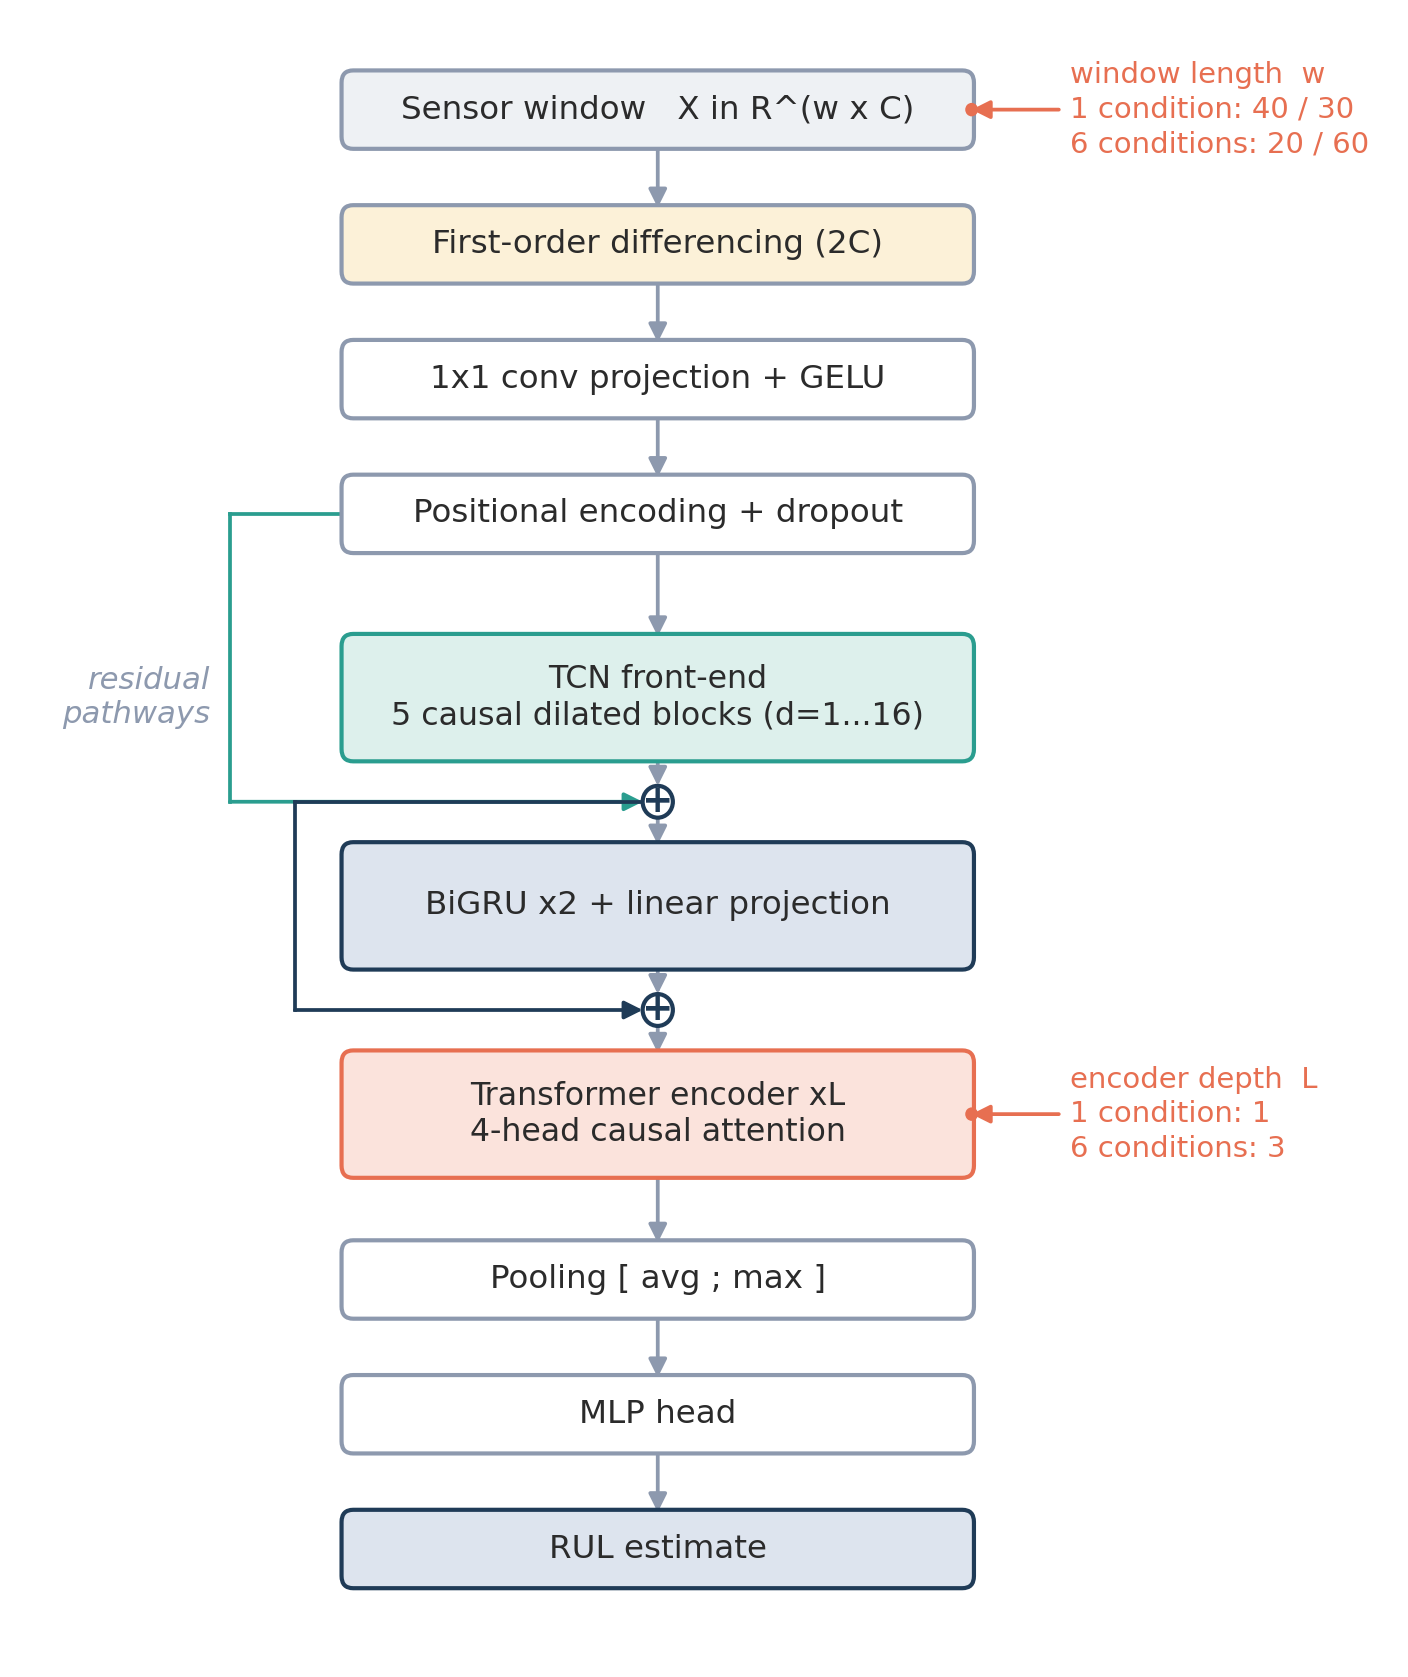
\includegraphics[width=\figarch]{../figures/raster_png_300dpi/fig1_architecture.png}
\caption{The hybrid model studied here. The two red notes give the window
length $w$ and encoder depth $L$ used for one and for six operating
conditions; the small circles mark where a residual branch rejoins the main
path. Section~\ref{sec:mechanism} asks why keeping these branches matters.}
\label{fig:arch}
\end{figure*}

\subsection{Five signs of a failed run}
\label{sec:collapse_def}

Call a run failed when its trained model predicts almost the same number for
every input. Five properties, each checkable from a run log or checkpoint,
identify it: (i) test prediction std $\sigma_{\hat y}<10^{-3}$ cycles, the
constant being 82.57 (FD002) and 82.97--83.00 (FD004); (ii) that constant
equals the training label mean $\bar y_{\mathrm{val}}$ to two decimals
(82.58 / 83.24); (iii) best validation RMSE is reached within 10--15 epochs,
never improves, and equals $\operatorname{std}(y_{\mathrm{val}})$ exactly
(41.97 / 42.24); (iv) because test engines are more degraded than validation
engines ($\bar y_{\mathrm{test}}=73.7$ versus 82.6 on FD002), test RMSE
follows from the label statistics as
\begin{equation}
\mathrm{RMSE}_{\mathrm{failed}}
= \sqrt{\operatorname{Var}(y_{\mathrm{test}})
        + \left(\bar{y}_{\mathrm{val}} - \bar{y}_{\mathrm{test}}\right)^{2}},
\label{eq:fingerprint}
\end{equation}
derived in Supplementary Section~S8; and (v) per-RUL-bucket errors follow the
constant prediction (69.9 / 38.5 / 10.7 / 38.2 on FD002).
Table~\ref{tab:fingerprint} checks (iv) against every failed run in the
archive: the prediction is accurate to 0.01 cycles on both subsets, so these
runs all end up at the same output rather than at a range of bad solutions.
Failed runs also give nearly identical RMSE across unrelated configurations
(43.848, 43.847, 43.846 for three depths and two GRL variants on FD002).
Losses fall smoothly, gradients behave and early stopping triggers normally,
so a reported ``RMSE = 43.85'' reads as poor tuning rather than as a distinct
failure. With one seed, a configuration that often fails cannot be told apart
from one that is simply mediocre.

\begin{table}[t]
\centering\footnotesize
\caption{A formula for the error of a failed run: observed versus predicted
RMSE (Eq.~(\ref{eq:fingerprint})).}
\label{tab:fingerprint}
\begin{tabularx}{\linewidth}{XCCCC}
\toprule
Subset & Std.\ $y_{\mathrm{val}}$ & Best-val & Constant pred./obs. &
Eq.~(\ref{eq:fingerprint}) / obs. \\
\midrule
FD002 & 41.97 & 41.97 & 82.58 / 82.57 & 43.85 / 43.85 \\
FD004 & 42.24 & 42.24 & 83.24 / 82.97--83.00 & 43.71 / 43.67--43.71 \\
\bottomrule
\end{tabularx}
\end{table}

\begin{figure}[t]
\centering
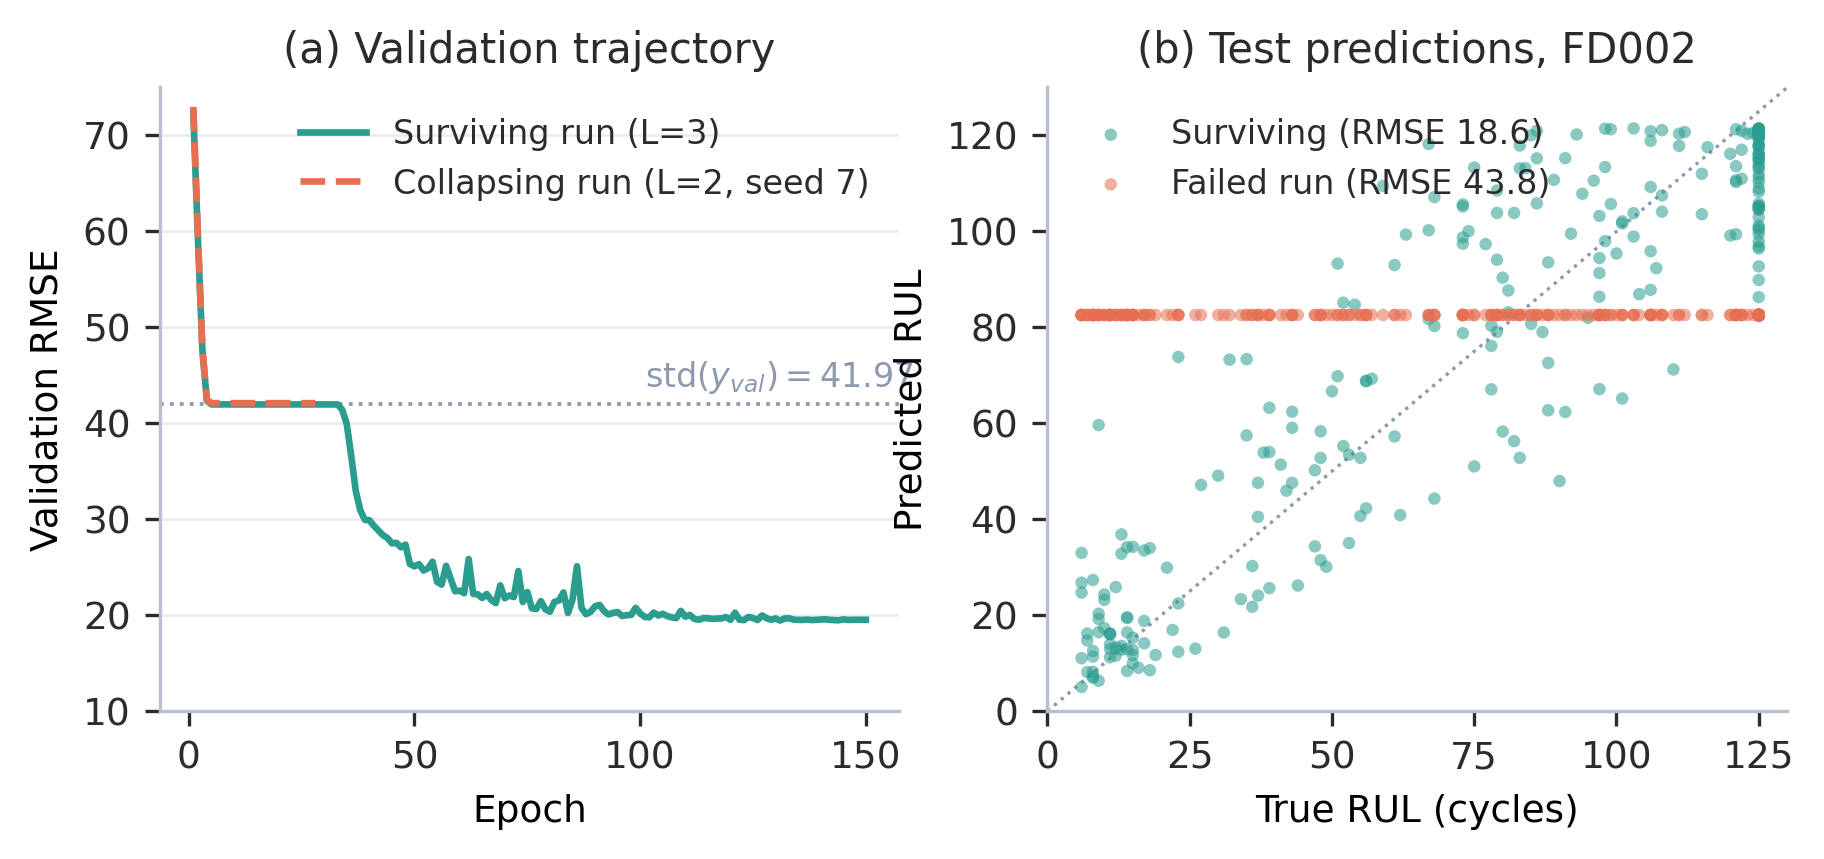
\includegraphics[width=0.68\linewidth]{../figures/raster_png_300dpi/fig2_fingerprint.png}
\caption{What a failed run looks like. (a) Validation RMSE of a working and
a failing FD002 run ($L{=}2$, seed 7): both sit at
$\operatorname{std}(y_{\mathrm{val}})$ for many epochs, and only the former
starts improving again near epoch 34. (b) Test predictions versus true RUL:
the failed model emits 82.6 for every engine.}
\label{fig:fingerprint_scatter}
\end{figure}

\subsection{How often it happens}
\label{sec:prevalence}

We audited all 161 archived runs, spanning $w\in\{20,30,40,60\}$,
$L\in\{1,\dots,4\}$, heads $h\in\{2,4,8\}$, three placements of adversarial
(GRL) regularisation and their controls; a run counts as failed iff test
RMSE $>40$, which Section~\ref{sec:collapse_def} shows to be conservative.
None of the 81 single-condition runs failed, including deliberately
pathological configurations (Table~\ref{tab:prevalence}). On multi-condition
data, failures gather in a few settings: in the controlled depth search
FD002 $L\in\{2,4\}$ failed while $L\in\{1,3\}$ trained normally, and the
order reversed on FD004 ($L{=}1$ failed, $L\geq2$ worked); window size and
head count behave similarly (FD002 with the adversarial backbone:
$w\in\{30,60\}$ failed, $w\in\{20,40\}$ did not; $h{=}2$ failed where
$h{=}4,8$ did not). Whether training works is a property of the dataset and
the architecture together, not of depth or window size alone. The complete
grids are in Supplementary Table~S2 and Fig.~S1.

\begin{table}[t]
\centering\footnotesize
\caption{How often runs failed on each subset (161 archived runs; four runs
with no recorded subset label are omitted from the breakdown).}
\label{tab:prevalence}
\begin{tabularx}{\linewidth}{Xccc}
\toprule
Subset & Runs & Failed & Rate \\
\midrule
FD001 (1 condition) & 45 & 0 & 0\% \\
FD003 (1 condition) & 36 & 0 & 0\% \\
FD002 (6 conditions) & 43 & 16 & 37.2\% \\
FD004 (6 conditions) & 33 & 8 & 24.2\% \\
\bottomrule
\end{tabularx}
\end{table}

The FD004 $w{=}60$, $L{=}3$ configuration has been trained under eight seeds:
six failed (43.67--43.72, each matching Eq.~(\ref{eq:fingerprint}) to two
decimals) and two worked (19.46, 19.60), with no intermediate outcome. The
two working runs form the tightest accuracy cluster in the archive (std
0.07), so one configuration can give first-quartile accuracy and still fail
on three retrains out of four. GRL variants shift which settings fail
without removing the problem, and seeded re-runs of archived failure cells
show that the seed, not the configuration alone, often decides the outcome
(Section~\ref{sec:dynamics}). How often a configuration fails therefore has
to be measured over seeds, as the audit of Section~\ref{sec:method_audit}
does. Published C-MAPSS results report one run per configuration;
best-of-$k$ tuning or reporting only the run that worked hides this.

\section{Why training fails}
\label{sec:mechanism}

We used two kinds of evidence: probes of nine saved checkpoints from the
controlled layer search (five failed, four working, plus two
single-condition references, where only $L$ or the seed changes), and
per-epoch records from six instrumented training runs
(Section~\ref{sec:dynamics}). We wanted to know what the internal features
of a failed model contain, what happens to its attention, and what separates
a failed seed from a working one at the same settings. Probe definitions,
per-checkpoint values and plots are in Supplementary Sections~S3--S4.

\subsection{What the internal features encode}
\label{sec:h1}

For each checkpoint we take the penultimate representation
$h\in\mathbb{R}^{256}$ on the test set, recover operating-condition labels by
$k$-means ($k{=}6$) on the three setting channels, and fit 5-fold
cross-validated linear and ridge probes for condition and RUL respectively.
Which condition an engine is running in is two to three times easier to read
off failed models (0.62--0.82) than off working ones (0.23--0.36), while RUL
readability falls from 0.66--0.76 to 0.04--0.09 on FD004 and from 0.78--0.81
to 0.55--0.58 on FD002 (Table~\ref{tab:mechanism}; full values in
Supplementary Table~S3 and t-SNE maps in Fig.~S2). The fixed output fits
this: per-condition label means on FD002 (86.7--87.1) and FD004 (92.7--93.3)
barely differ from the overall means, so features that carry only condition
have nothing better to output than the mean. On FD004 a failed model removes
the RUL signal from $h$ altogether; on FD002 a linear RUL component survives
even though the prediction is still 82.57, because the attention stack has
flattened the sequence. What fails is the usable representation, not simply
the information a linear probe can extract.

\subsection{What happens to attention}
\label{sec:h2}

For every layer of every checkpoint we compute the normalised entropy of the
causal attention distributions, averaged over heads, queries and test
samples, where 1.0 means every time step weighted equally. Every failed
checkpoint sits at 1.0000 to four decimals, with the largest weight at its
uniform value, while working models lie between 0.70 and 0.93
(Table~\ref{tab:mechanism}; Supplementary Table~S4 and Fig.~S3). Working
multi-condition models sharpen with depth (FD002-L3: 0.84, 0.77, 0.70),
concentrating on positions that matter for wear; failed ones never
distinguish positions. Flat attention on its own is not the problem: the
single-condition references (FD001 0.89, FD003 0.93) are the flattest
working models in the archive and predict well, because their TCN/GRU
residual branches carry the degradation signal regardless of attention. The
damaging combination is flat attention, features organised by condition and
a fixed output. Flat attention describes how the condition cue stops the
model from using time, rather than causing the failure by itself.

\begin{table*}[t]
\centering\footnotesize
\caption{Evidence from the probes, pooled over checkpoints: how well condition
and RUL can be read from the internal features, mean normalised attention
entropy, and output std. Per-checkpoint values are in Supplementary
Tables~S3--S4.}
\label{tab:mechanism}
\begin{tabularx}{\linewidth}{Xcccc}
\toprule
Checkpoints & Cond.\ acc. & RUL $R^2$ (FD002 / FD004) & Entropy & Pred.\ std \\
\midrule
Failed runs (5) & 0.62--0.82 & 0.55--0.58 / 0.04--0.09 & 1.0000 & $<10^{-3}$ \\
Working, multi-cond. (6) & 0.23--0.36 & 0.76--0.81 / 0.66--0.76 & 0.70--0.93 & --- \\
Working, single-cond. (2) & n/a & 0.81--0.87 & 0.89--0.93 & --- \\
\bottomrule
\end{tabularx}
\end{table*}

\subsection{What decides whether a run recovers}
\label{sec:dynamics}

The two sections above describe the end state. To see what separates a failed
seed from a working one at the same settings, six instrumented re-runs
recorded, each epoch, the gradient $L_2$ norms of the TCN, GRU, attention and
head groups, attention entropy, condition- and RUL-probe accuracy on a fixed
batch, and validation RMSE (protocol in Supplementary Section~S1). The
result changed our reading. A failed run has not fallen into a bad solution
of its own; it has failed to get out of a stage that every run passes
through. All six, including the five that ended well, first settle at the
constant output of Section~\ref{sec:collapse_def}: validation RMSE pinned at
$\operatorname{std}(y_{\mathrm{val}})$, entropy exactly 1.0, prediction std
near zero, for 16--34 epochs (Table~\ref{tab:escape}). What differs is what
happens next.

In all five working runs the recovery follows the same order. The
pre-clipping TCN gradient norm jumps by two orders of magnitude
($\times$129--235) within 1--3 epochs while the encoder gradient stays
flat; attention entropy drops below 1.0 for the first time (0.93--0.99) and
keeps falling; and condition-probe accuracy falls from 0.48--0.70 to
0.29--0.40 as the RUL probe rises. Before recovery the encoder gradient
decays monotonically ($102\to1.2$ over 37 epochs in FD002 $L{=}2$, seed 42),
since a fixed output gives attention no error signal. Recovery happens at
epochs 21--39 and overlaps the early-stopping horizon (patience 20 from a
flat stretch starting near epoch 5--10): working runs get there only because
tiny improvements in validation RMSE ($41.975\to41.971\to\dots$)
intermittently reset the patience counter. Archived failed runs stopped at
epochs 31--38, inside that window, so some may have been recoveries cut
short by the stopping rule. Two seeded re-runs show how much the seed
matters: FD002 $L{=}2$ recovered under seed 42 (19.04) but failed under seed
7 (43.87), and FD004 $L{=}1$, archived as failed, recovered under the
instrumented protocol (20.92), which also varied the train/val split. What
looked like settings that always fail are in fact settings where either
outcome is likely, depending on the seed. Because the flat stretch is
visible from epoch $\approx$5, tens of epochs before early stopping, it gives
a third check for the procedure of Section~\ref{sec:method_audit}.

\begin{table}[t]
\centering\footnotesize
\caption{When the six instrumented runs started to improve again. Flat and
Recovery are epoch numbers; TCN jump is the pre-clipping gradient-norm ratio
at that point.}
\label{tab:escape}
\begin{tabularx}{\linewidth}{XCCCCC}
\toprule
Run & Final RMSE & Outcome & Flat (ep.) & Recovery & TCN jump \\
\midrule
FD002 $L{=}2$, s42 & 19.04 & recovered & 34 & 39 & $\times$163 \\
FD002 $L{=}3$, s42 & 18.58 & recovered & 30 & 34 & $\times$150 \\
FD002 $L{=}2$, s7 & 43.87 & failed & 25 & never & --- \\
FD004 $L{=}1$, s42 & 20.92 & recovered & 16 & 21 & $\times$129 \\
FD004 $L{=}3$, s42 & 19.60 & recovered & 26 & 31 & $\times$235 \\
FD004 $L{=}3$, s123 & 20.49 & recovered & 32 & 37 & $\times$169 \\
\bottomrule
\end{tabularx}
\end{table}

\begin{figure}[t]
\centering
\includegraphics[width=0.72\linewidth]{figures/fig5_escape_race.png}
\caption{What separates a working run from a failed one, across six
instrumented runs. (a) Validation RMSE: all runs sit at
$\operatorname{std}(y_{\mathrm{val}})$ for a long stretch, and working runs
start improving at staggered epochs. (b) Attention entropy: exactly 1.0
during the flat stretch, dropping only when training recovers. (c) TCN
gradient norm (log scale): a hundredfold jump. (d) Condition-probe accuracy:
high during the flat stretch, falling sharply once training recovers.}
\label{fig:escape}
\end{figure}

\subsection{Putting the pieces together}
\label{sec:synthesis}

The evidence fits one account. From near-random initialisation, the quickest
way to reduce MSE before the inputs have been decoded is to output the label
mean; every audited multi-condition run reaches this fixed output within a
few epochs and stays there for 16--34 epochs. With six operating conditions
the features around it are organised by which condition the engine is in
(Section~\ref{sec:h1}); with a fixed output the attention branch gets no
error signal and ends up weighting every time step equally
(Section~\ref{sec:h2}); training then resumes only after a sudden jump in
the gradients of a residual branch, usually the TCN, which lets attention
work again and replaces the condition cue with task information
(Section~\ref{sec:dynamics}). Whether that happens before early stopping
depends on window length, depth and seed, which gives the pattern we see:
settings that train reliably, settings that usually fail (FD002
$L\in\{2,4\}$), and settings where the seed decides (FD004 $w{=}60$,
$L{=}3$: six of eight failed).

Two more observations complete the picture. Single-condition data is
unaffected because the operating settings are constant channels removed by
the variance filter: there is no condition cue to pick up, and the TCN/GRU
branches suffice even when attention is nearly flat (FD003: 0.93). The
component removals supply the causal complement (full table in
Supplementary Table~S6): taking out the TCN front end makes FD002 fail
(19.73 $\to$ 43.84) but only degrades FD004 ($\to$ 24.21), whereas taking
out the Transformer encoder or the difference features makes FD004 fail
($\to$ 43.68 / 43.73) and leaves FD002 well. Which branch the model depends
on changes with window length and condition count, and keeping more than one
usable branch is what makes training reliable. Fig.~\ref{fig:phase} sketches
the pattern that Section~\ref{sec:method} turns into rules.

\begin{figure}[t]
\centering
\includegraphics[width=0.60\linewidth]{figures/fig6_phase_diagram.png}
\caption{Which settings train reliably. Horizontal axis: how much the six
operating conditions change the sensor readings. Vertical axis: how often a
run starts improving again before early stopping (points at measured rates
with pooled run counts). The three regions are settings that train reliably
for every seed, settings that depend on the seed, and settings that usually
fail.}
\label{fig:phase}
\end{figure}

\section{Rules for training reliably}
\label{sec:method}

The pattern in Section~\ref{sec:synthesis} suggests a straightforward
procedure, which we call CAS-Fuse. Four rules choose the settings that
trained reliably in the audit; two more keep several branches of the model
able to carry the degradation signal; and a short check after training
catches the seed dependence that no choice of architecture removes.

\subsection{How to set up the model}

\paragraph{Rule 1: window length by number of conditions} Window length
controls how many condition changes a training window averages over.
Single-condition subsets are insensitive to $w$; multi-condition subsets
were fragile in the audited mid-range (FD002 at $w\in\{30,60\}$, FD004 at
$w{=}40$). We use $w=40$ (FD001), $w=30$ (FD003) and the audited extremes
($w=20$ on FD002, $w=60$ on FD004).

\paragraph{Rule 2: depth by number of conditions} Changing depth does not
have the same effect at every condition count (Supplementary Table~S2):
FD002 $L\in\{2,4\}$ fail and $L\in\{1,3\}$ work; on FD004 $L{=}1$ fails
while $L\geq2$ works. We set $L=1$ for single-condition data and $L=3$ for
multi-condition data, outside the FD002 even-depth band that failed. The
resulting models have 1.08\,M and 1.47\,M parameters; all other
hyperparameters are shared, so $w$ and $L$ are the only choices that adapt.

\paragraph{Rule 3: keep more than one usable branch} The TCN front end,
difference augmentation and BiGRU stage stay in even where they add little
accuracy, because each is the branch the model depends on somewhere in the
range of condition structures: the TCN for short windows with many
conditions, attention over explicit rate signals for long windows with many
conditions, and the GRU as a residual backup. In every instrumented run it
was the convolutional branch that powered the recovery
(Section~\ref{sec:dynamics}). With several usable branches, failure needs
several independent things to go wrong at once.

\paragraph{Rule 4: keep the parts attention needs} Sinusoidal positional
encoding and sensor-channel dropout are retained: removing positional
encoding degraded mean RMSE by 16.9\% and raised the FD001 val--test gap from
17.5\% to 288.6\%; removing sensor dropout cost 3.1\% mean RMSE.

\subsection{What we removed, and why}
\label{sec:method_prune}

Three popular components were dropped on experimental grounds (full
removals in Supplementary Table~S6). Gradient reversal
\cite{ganin2016domain} looks like the answer to a condition cue and is
empirically the wrong one: it moves the failing settings around rather than
shrinking their number, helps by $\le$1.5 RMSE on single-condition data
where it is unnecessary, and injects condition-discriminating gradients into
the features most at risk of being picked up. Global and condition-aware
contrastive losses \cite{ragab2022contrastive} both made FD002 fail (43.46 /
43.49), since same-state pairs are rare under six interleaved regimes.
Removal A5 shows avg-only pooling slightly more accurate than the dual head
(16.43 versus 17.27 mean RMSE), but we keep the dual head because the
five-seed audit ran on this exact architecture; changing it would invalidate
the audit for a 4.9\% gain of unverified reliability. When reliability
matters, evidence about training should decide which components stay, not
only the accuracy difference.

\subsection{Checking a trained model}
\label{sec:method_audit}

No choice of settings removes seed dependence: the FD004 configuration from
Rules 1--2 failed on six of eight seeds while giving first-quartile accuracy
on the other two. The following checks are therefore part of the method,
and they are cheap.

\begin{enumerate}
  \item \emph{Train with $k\geq3$ seeds} (we use 5). This is the only step
        needing compute beyond standard practice.
  \item \emph{Check A: prediction std and Eq.~(\ref{eq:fingerprint}).}
        Flag if $\sigma_{\hat y}<0.01$ cycles, or if test RMSE matches the
        value the formula gives for a fixed output. One forward pass.
  \item \emph{Check B: attention entropy.} Flag if mean normalised entropy
        exceeds 0.99 (working 0.70--0.93; failed 1.0000). One hooked
        forward pass.
  \item \emph{Check C: a long flat stretch during training.} Flag a run as
        at risk when validation RMSE sits within $\varepsilon$ of
        $\operatorname{std}(y_{\mathrm{val}})$ with prediction std $<0.1$
        for $N$ consecutive epochs. The flat stretch is visible from epoch
        $\approx$5 and recovery happens by epoch 40, so at-risk runs can be
        stopped and started again with a new seed well before early stopping.
  \item \emph{Report mean $\pm$ std over working seeds together with the
        failure rate.} A configuration above a set threshold (we use 1/5) is
        rejected whatever its best-seed accuracy. On FD004, where every
        audited configuration depends on the seed, the procedure starts
        again with a new seed until Checks A--C pass, and reports the
        statistics of the runs that worked (19.53 $\pm$ 0.07 over two of
        eight).
\end{enumerate}

\subsection{What the rules do not promise}
\label{sec:method_tradeoff}

CAS-Fuse does not chase per-subset state-of-the-art accuracy; specialised
architectures reach lower single-run RMSE (Supplementary Table~S5). Within
the hybrid models used in applied RUL work, the claim is the best verified
reliability at competitive accuracy, together with an account of why the
rules work.

\section{Experiments}
\label{sec:experiments}

\subsection{Protocol}

C-MAPSS FD001--FD004 are used with the preprocessing of
Section~\ref{sec:phenomenon} (cap 125, min--max by training statistics,
85/15 train/val window split, last-window test). Metrics are test RMSE
(primary), the asymmetric PHM08 score \cite{saxena2008damage}, $R^2$, and
the failure rate over seeds as flagged by Section~\ref{sec:method_audit}.
Every configuration from Rules 1--4 is trained with five seeds (42, 7, 123,
2026, 3407) controlling initialisation and data order; FD004 additionally
pools four archived runs of the same configuration. We report mean $\pm$ std
over working seeds alongside the failure rate; no C-MAPSS comparison table
we found reports either quantity. Training used an Apple M-series GPU (MPS)
and PyTorch 2.8, at 60--350\,min per run; the 20-run audit took about two
days on one consumer device, and instrumented runs add 50--100\% overhead.
Full settings, the seed-by-seed ledger and the reproducibility file map are
in Supplementary Sections~S1 and~S7.

\subsection{Do the rules hold across seeds}

\begin{table}[t]
\centering\footnotesize
\caption{How often runs failed: (i) the archived runs across all model
variants and (ii) the Rules 1--4 configuration with five seeds per subset.}
\label{tab:audit}
\begin{tabularx}{\linewidth}{Xcccc}
\toprule
Configuration family & FD001 & FD002 & FD003 & FD004 \\
\midrule
Archive, all labelled variants (157 runs) & 0/45 & 16/43 & 0/36 & 8/33 \\
Rules 1--4, five seeds & 0/5 & 0/5 & 0/5 & 6/8 \\
\bottomrule
\end{tabularx}
\end{table}

On FD001, FD002 and FD003 the chosen settings worked in all fifteen runs,
with per-seed RMSE tight enough for mean $\pm$ std to be meaningful:
13.66 $\pm$ 0.10, 19.43 $\pm$ 0.44 and 16.09 $\pm$ 0.52
(Table~\ref{tab:audit}, Fig.~\ref{fig:seeds}). On FD004 the seed decides: six
of eight runs ended at the fixed output predicted by
Eq.~(\ref{eq:fingerprint}), while the two that worked reached 19.46/19.60
(std 0.07), with nothing in between. The rules remove the settings that
always failed (FD002: 37\% in the archive, 0/5 here) but cannot make every
seed work everywhere; the checks in Section~\ref{sec:method_audit} catch the
remaining failures in minutes and let us start a fresh run. No audited FD004
configuration trained reliably over multiple seeds, so this looks like a
property of that region rather than of one poor rule.

\begin{figure}[t]
\centering
\includegraphics[width=0.56\linewidth]{figures/fig9_seed_boxplot.png}
\caption{Per-seed test RMSE for the Rules 1--4 configuration (teal circles =
working runs; coral crosses = failed runs; navy line = mean of the working
runs). FD004 splits into two groups: six seeds at 43.67--43.72, two at
19.46--19.60, nothing in between.}
\label{fig:seeds}
\end{figure}

\subsection{Accuracy, score, and component removals}

The chosen configuration beats a vanilla Transformer on every subset and
sits in the DCNN/BiGRU-TSAM/MS-DCNN band, but stays below specialised
architectures such as DKAMFormer \cite{kim2025dkam}, which targets
FD002/FD004 with dedicated multi-scale machinery. The full comparison
against twelve published methods is in Supplementary Table~S5; none of
those rows reports a failure rate. Mean PHM08 scores over working seeds are
307 (FD001), 2\,855 (FD002), 1\,050 (FD003) and 1\,783--2\,448 (FD004),
against 61\,569--75\,860 for failed runs. The asymmetric penalty therefore
multiplies the fixed-output failure by 15--250$\times$ relative to RMSE,
which is why Score, not RMSE, is the metric that matters in service.

The eight-way component removal (A0--A7, four subsets, with PHM08 scores
recomputed from saved checkpoints) is in Supplementary Table~S6. Read
alongside Section~\ref{sec:mechanism}, it carries much of the causal
argument: taking out a branch the model was thought to depend on (A1 on
FD002; A3/A4 on FD004) produces the same fixed-output failure confirmed by
Eq.~(\ref{eq:fingerprint}), rather than a graceful loss of accuracy, whereas
an accuracy-only reading would rank A5, where removing max pooling improves
the mean, as the best change. The instrumented runs supply the complement:
recovery is driven by the TCN branch (a hundredfold gradient jump,
$\times$129--235), the same branch whose removal forces FD002 to fail for
good.

Supplementary Sections~S5--S6 also give the segment-error signature on every
subset (FD002: 69.9 / 38.5 / 10.7 / 38.2 across RUL buckets $<30$, 30--60,
60--100, $\geq100$), the val--test gaps of working runs ($-2.3$\% to
$+25.3$\%, largest on FD003, a known limitation of windowed splits retained
for comparability), and the layer-1 attention maps (mean normalised row
entropy 0.7221 for a working checkpoint against exactly 1.0000 for a failed
one).

\section{Discussion}
\label{sec:discussion}

What happens in a failed run is easy to misread. Loss falls smoothly, so it
is not divergence; the val--test gap is small, so it is not overfitting; and
it is not the attention problem reported for vision Transformers
\cite{zhai2023stabilizing}, where attention sharpens too early. Here it
flattens until every time step is weighted equally. The network has found
the simplest way to reduce MSE, which is to output the label mean, and then
never leaves before the learning-rate budget and early-stopping patience run
out. The failure is hard to spot because that answer is moderately good
under the training loss; only the score used in service and the checks of
Section~\ref{sec:method_audit} reveal it.

\subsection{Limitations}

All quantitative statements come from C-MAPSS. The explanation is framed in
terms of architecture and data structure, but whether it carries over to
N-CMAPSS, milling or bearing run-outs is a hypothesis, not a result. Rules
1--2 were read off one set of experiments rather than derived from theory,
and the FD004 result shows that local rules cannot guarantee reliable
training even within one benchmark. Five seeds per configuration is more
than is usually reported, but it is still a coarse estimate of a failure
probability near 0 or 1; the 6/8 FD004 rate has a wide binomial interval.
Our audit holds the train/val split fixed across seeds, matching the
archived runs, while the instrumented study also varied it and outcomes
changed (FD004, seed 123: failed under the fixed split, worked under the
varied split); the ``seed'' whose reliability one audits should include the
split. Windowed train/val splits from the same trajectories also inflate
validation optimism relative to engine-holdout splits, at the cost of
val--test gaps up to 25\% on FD003.

\subsection{Practice and outlook}

The checks are not tied to our architecture. Report mean $\pm$ std over at
least three seeds together with the failure rate, and treat best-of-$k$
tuning as suspect by default. Record two numbers during training, prediction
std on a held-out batch and mean attention entropy, whose thresholds are
sharp (0.01 cycles; 0.99); watch for a validation RMSE that sits at
$\operatorname{std}(y_{\mathrm{val}})$ with near-constant predictions, which
means the run is still printing the average and should be started again with
a new seed or given more patience. Keep more than one usable temporal branch,
since removing one for the sake of a smaller model should require evidence
that training is unaffected, not just that accuracy is; and judge the
deployed model on the asymmetric score. If recovery depends on a jump in the
TCN gradients, warm-up schedules or a learning-rate increase triggered by a
long flat stretch might make the seed-dependent settings train reliably; the
per-epoch records give a way to test that, and the same checks apply to any
sensor-regression task with several operating conditions.

\section{Conclusion}
\label{sec:conclusion}

We documented, and partly fixed, a training failure in the hybrid deep
models used for aero-engine RUL prediction on multi-condition data. Across
161 runs, 37.2\% of FD002 and 24.2\% of FD004 runs ended by predicting one
fixed number for every engine, whose test error can be computed in closed
form; none of 81 single-condition runs did. Every run first spends time
printing the training-set average, with features organised by operating
condition and attention weights identical at every time step. Training
starts to improve again only when gradients in the convolutional branch jump
about a hundredfold, and this has to happen before early stopping. The rules
we propose choose window length and depth by the number of operating
conditions, keep several usable branches, drop the adversarial and
contrastive components, and add three cheap checks; over five seeds they
trained reliably on FD001/FD002/FD003 (13.66/19.43/16.09 RMSE), while on
FD004 six of eight runs still failed and the two that worked agreed at
19.53 $\pm$ 0.07, which the checks catch in time to start again. A table of
single-run accuracies cannot say whether a model is fit for safety-critical
use: one that may, on retraining, quietly turn into a device printing the
fleet-average RUL for every engine is not usable at any RMSE. That
probability has almost never been measured; we supply the measurement, the
explanation and the rules.


%% numeric style emulated via thebibliography (tectonic 0.14 has no bibtex)
{\small\begin{thebibliography}{99}

\bibitem{jardine2006review} Jardine, A., Lin, D. and Banjevic, D.. ``A review on machinery diagnostics and prognostics implementing condition-based maintenance.'' Mechanical Systems and Signal Processing 20(1), 148--181, 2006.
\bibitem{saxena2008damage} Saxena, A., Goebel, K., Simon, D. and Eklund, N.. ``Damage propagation modeling for aircraft engine run-to-failure simulation.'' In International Conference on Prognostics and Health Management (PHM), 1--9, 2008.
\bibitem{lei2018machinery} Lei, Y., Li, N., Guo, L., Li, N., Yan, T. and Lin, J.. ``Machinery health prognostics: a systematic review from data acquisition to RUL prediction.'' Mechanical Systems and Signal Processing 104, 799--834, 2018.
\bibitem{hu2022prognostics} Hu, Y., Miao, X., Si, Y., Pan, E. and Zio, E.. ``Prognostics and health management: a review from the perspectives of design, development and decision.'' Reliability Engineering \& System Safety 217, 108063, 2022.
\bibitem{babu2016deep} Babu, G., Zhao, P. and Li, X.. ``Deep convolutional neural network based regression approach for estimation of remaining useful life of machines.'' In International Conference on Database Systems for Advanced Applications (DASFAA), 214--228, 2016.
\bibitem{li2018remaining} Li, X., Ding, Q. and Sun, J.. ``Remaining useful life estimation in prognostics using deep convolution neural networks.'' Reliability Engineering \& System Safety 172, 1--11, 2018.
\bibitem{zheng2017long} Zheng, S., Ristovski, K., Farahat, A. and Gupta, C.. ``Long short-term memory network for remaining useful life estimation.'' In IEEE International Conference on Prognostics and Health Management (ICPHM), 88--95, 2017.
\bibitem{yuan2016fault} Yuan, M., Wu, Y. and Lin, L.. ``Fault diagnosis and remaining useful life estimation of aero engine using LSTM neural network.'' In IEEE International Conference on Aircraft Utility Systems (AUS), 135--140, 2016.
\bibitem{xiang2021multicellular} Xiang, S., Qin, Y. and Luo, J.. ``Multi-cellular LSTM deep learning model for aero-engine remaining useful life prediction.'' Reliability Engineering \& System Safety 216, 107927, 2021.
\bibitem{wang2024dvgtformer} Wang, L., Cao, H., Ye, Z., Xu, H. and Yan, J.. ``DVGTformer: a dual-view graph Transformer to fuse multi-sensor signals for remaining useful life prediction.'' Mechanical Systems and Signal Processing 207, 110935, 2024.
\bibitem{zhang2024tatfa} Zhang, Y. and others. ``TATFA-Transformer: trend-aware temporal feature attention Transformer for aero-engine RUL prediction.'' TODO-VERIFY , 2023. [TODO-VERIFY]
\bibitem{kim2025dkam} authors, D.. ``DKAMFormer: domain knowledge-augmented multiscale Transformer for remaining useful life prediction of aeroengine.'' IEEE/CAA Journal of Automatica Sinica , 2025. DOI: 10.1109/JAS.2025.125126. [TODO-VERIFY]
\bibitem{bai2018empirical} Bai, S., Kolter, J. and Koltun, V.. ``An empirical evaluation of generic convolutional and recurrent networks for sequence modeling.'' arXiv preprint arXiv:1803.01271 , 2018.
\bibitem{vaswani2017attention} Vaswani, A., Shazeer, N., Parmar, N. and others. ``Attention is all you need.'' In Advances in Neural Information Processing Systems (NeurIPS), 5998--6008, 2017.
\bibitem{zhang2022prediction} Zhang, J., Jiang, Y., Wu, S., Li, X., Luo, H. and Yin, S.. ``Prediction of remaining useful life based on bidirectional gated recurrent unit with temporal self-attention mechanism.'' Reliability Engineering \& System Safety 221, 108297, 2022.
\bibitem{cnnlstmsam2019li} authors, C.. ``Aero-engine RUL prediction with CNN-LSTM and self-attention mechanism.'' TODO-VERIFY , 2019. [TODO-VERIFY]
\bibitem{vaetransformer2022} authors, V.. ``Variational autoencoder enhanced Transformer for remaining useful life prediction.'' TODO-VERIFY , 2022. [TODO-VERIFY]
\bibitem{liu2021clustering} Liu, J., Lei, F. and Pan, C.. ``Prediction of remaining useful life of multi-stage aero-engine based on clustering and LSTM fusion.'' International Journal of System Assurance Engineering and Management , 2021. [TODO-VERIFY]
\bibitem{ganin2016domain} Ganin, Y., Ustinova, E., Ajakan, H. and others. ``Domain-adversarial training of neural networks.'' Journal of Machine Learning Research 17(59), 1--35, 2016.
\bibitem{ragab2022contrastive} Ragab, M., Chen, C., Wu, M., Kwoh, C., Li, X. and Zhu, Y.. ``Contrastive adversarial domain adaptation for machine remaining useful life prediction.'' IEEE Transactions on Industrial Informatics 18(5), 3502--3512, 2022.
\bibitem{geirhos2020shortcut} Geirhos, R., Jacobsen, J., Michaelis, C., Zemel, R., Brendel, W., Bethge, M. and Wichmann, F.. ``Shortcut learning in deep neural networks.'' Nature Machine Intelligence 2, 665--673, 2020.
\bibitem{sturm2012clever} Sturm, J. and Others. ``Clever Hans.'' In ICML Workshop on Robot Learning, 2012. [TODO-VERIFY]
\bibitem{zhai2023stabilizing} Zhai, S., Likhomanenko, T., Littwin, E., Busbridge, D., Ramapuram, J., Zhang, Y., Gu, J. and Susskind, J.. ``Stabilizing Transformer training by preventing attention entropy collapse.'' In International Conference on Machine Learning (ICML), 2023.
\bibitem{dong2021attention} Dong, Y., Cordonnier, J. and Loukas, A.. ``Attention is not all you need: pure attention loses rank doubly exponentially with depth.'' In International Conference on Machine Learning (ICML), 2021.
\bibitem{chen2021exploring} Chen, X. and He, K.. ``Exploring simple Siamese representation learning.'' In IEEE/CVF Conference on Computer Vision and Pattern Recognition (CVPR), 2021.
\bibitem{grill2020bootstrap} Grill, J., Strub, F. and Altch\'e. ``Bootstrap your own latent: a new approach to self-supervised learning.'' In Advances in Neural Information Processing Systems (NeurIPS), 2020.
\end{thebibliography}}

\end{document}
